\section{单标记数据分析}
对于单标记一侧的分析,如果在重建一个$\lambdacpm$ 的衰变道过程中有了多个候选者,我们选择一个具有最小的$|\Delta{}E|$的候选者保留下来。
当我们通过初步的事例筛选,且对$\Delta{}E$做了相应要求,每一个衰变道拿到了相应的候选事例,然后我们通过拟合$M_{\rm BC}$的分布来提取信号和本底的数目。
我们对于数据和MC采用的拟合方法均为不分区间的极大似然拟合。
把产额和效率作为待测参数通过拟合来提取。
图~\ref{fig:ST_datafit}给出了数据中每个道的拟合结果,我们是把电荷共轭道的$\lambdacp$和$\lambdacm$合并在一起来进行估计的。
拟合区间为~[2.25,2.3]$\gevcc$。 
在每一个道的拟合函数中都包含着两部分,信号形状和本底形状。
图中黑色的带误差的点是数据,红线是总的拟合线,绿色的虚线是信号的形状,蓝色的虚线是用来描述本底的ARGUS函数~\cite{ref:argus}。
信号形状我们采用来自于单标记的信号形状MC卷积一个高斯函数来描述。
高斯函数用于描述由于束流能量($E_{\rm beam}$)测量不够准确给~$M_{\rm BC}$ 带来的偏移以及~MC 和数据的分辨差异,其中心值和宽度都是浮动的。
ARGUS本底函数的具体表达式为:
\begin{equation}
f(m;m_{0},\xi)=Am(1-\frac{m^{2}}{m^{2}_{0}})^{0.5} e^{\xi(1-\frac{m^{2}}{m_{0}^{2}})}.
\end{equation}
其中,$A$ 是归一化系数;$m$ 是要拟合的量(即~$M_{\rm BC}$);$m_{0}$ 是右端的截断值,对于~$M_{\rm BC}$ 而言,其右端的截断值应该等于~$e^{+}e^{-}$ 束流的平均能量~$E_{\rm beam}$,在拟合时我们将~$m_{0}$ 固定为$2.3$;$\xi$ 是另一个浮动参数,通过拟合获得。
我们抽取$M_{\rm BC}$在$(2.282, 2.291)\gevcc$之间的事例产额作为该衰变道单标记的事例数$N_{i}^{ST}$。

为了获取单标记侧信号过程的筛选效率,也同时考虑到要降低系统误差的需求,我们在对MC拟合之前先考虑了MC样本和数据样本在$\Delta E$和$M_{\rm BC}$谱分辨上的差异。
利用图~\ref{fig:ST_datafit}拟合$M_{\rm BC}$谱过程中给出来的高斯分辨参数我们可以知道现有MC样本和数据样本之间在分辨上的差异。
为了拿到在$\Delta E$谱上MC和数据在分辨上的差异,我们对数据中$\Delta E$的分布也进行了拟合。

在拿到$\Delta E$和$M_{\rm BC}$谱上MC数据之间的分辨函数之后,我们按照这一参数对现有MC的$\Delta E$和$M_{\rm BC}$谱进行修正,使其分辨和数据尽可能的一致。
所谓的修正就是按照拟合得到的分辨函数去弥散原始MC的分布。
用这份修正过的MC样本加上Cocktail MC中的其他过程,生成一份新的Cocktail MC。
然后利用和数据完全类似的拟合方法来拟合这份新的Cocktail MC样本来得到单标记的选择效率。
图~\ref{fig:ST_cockmcfit}是拟合结果图。MC的拟合依然是合并了$\lambdacp$和$\lambdacm$的衰变的。
我们将具体的单标记产额值和效率值列在表~\ref{tab:STyields}中。
分别对应公式\ref{eq:st}中的$N_{i}^{ST}$和$\varepsilon_{i}^{ST}$。
这些效率值是不包含表~\ref{tab:interDecay}中的次级衰变分支比的。

%%%%%%%%%%%%%%%%%%%%%%%%%%%%%%%%%%%%%%%%%%%%%%%%%%%%%%%%%%%%%%%%%%%%%%%%%%%%%%%%%%%%%%%%%
\begin{figure*}[]
\centering
\subfigure[]
{
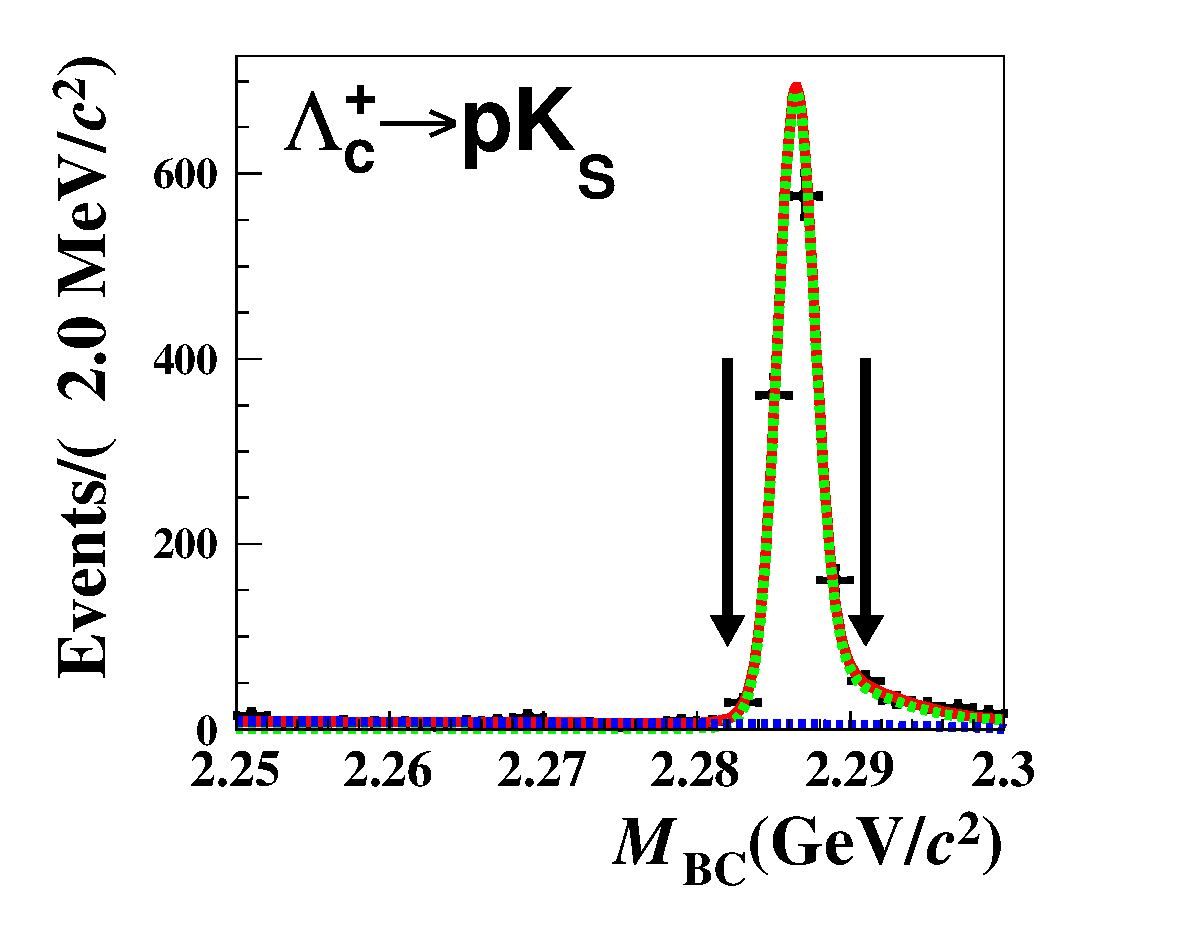
\includegraphics[width=0.3\textwidth]{chap2_ST_data_mode0}
}
\hspace{1pt}
\subfigure[]
{
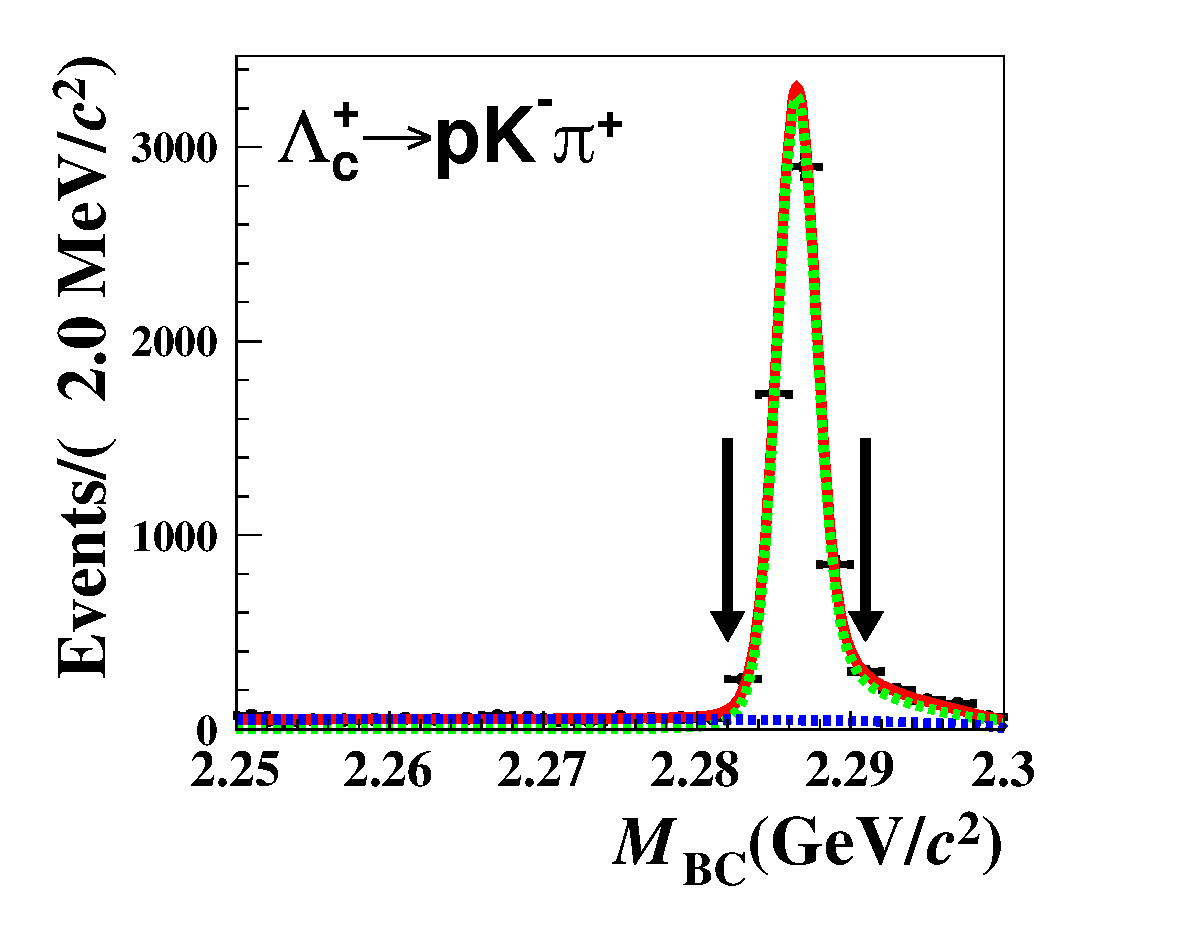
\includegraphics[width=0.3\textwidth]{chap2_ST_data_mode1}
}
\hspace{1pt}
\subfigure[]
{
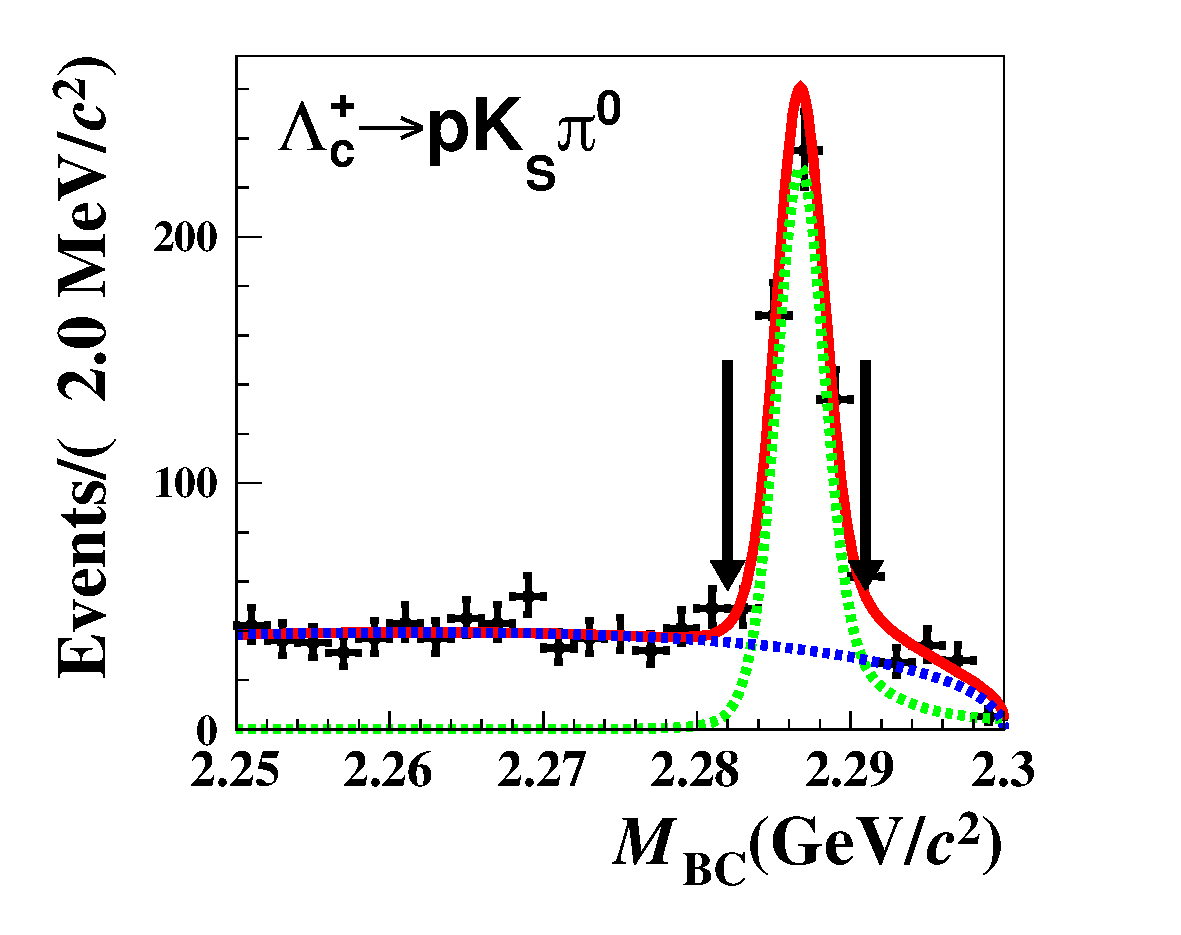
\includegraphics[width=0.3\textwidth]{chap2_ST_data_mode2}
}
\hspace{1pt}
\subfigure[]
{
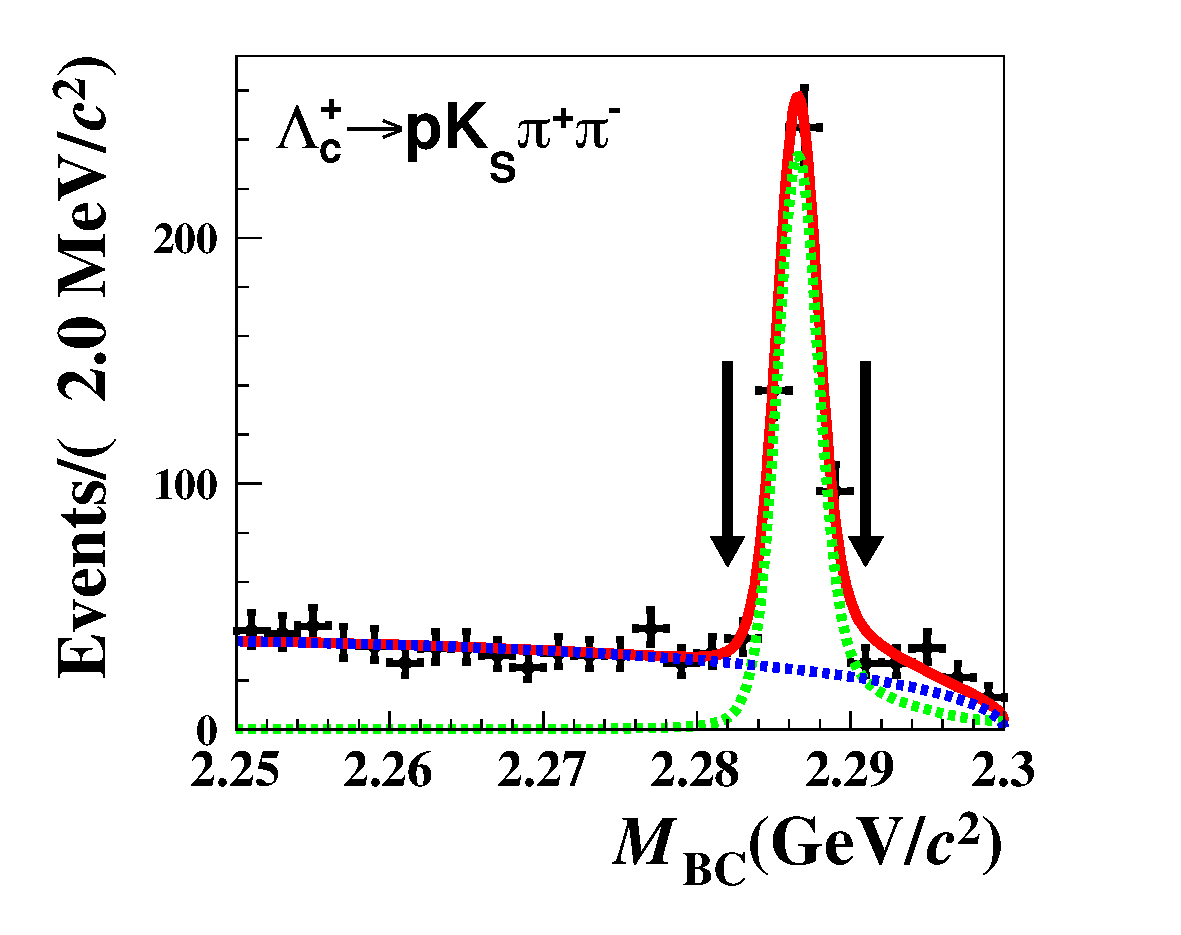
\includegraphics[width=0.3\textwidth]{chap2_ST_data_mode3}
}
\hspace{1pt}
\subfigure[]
{
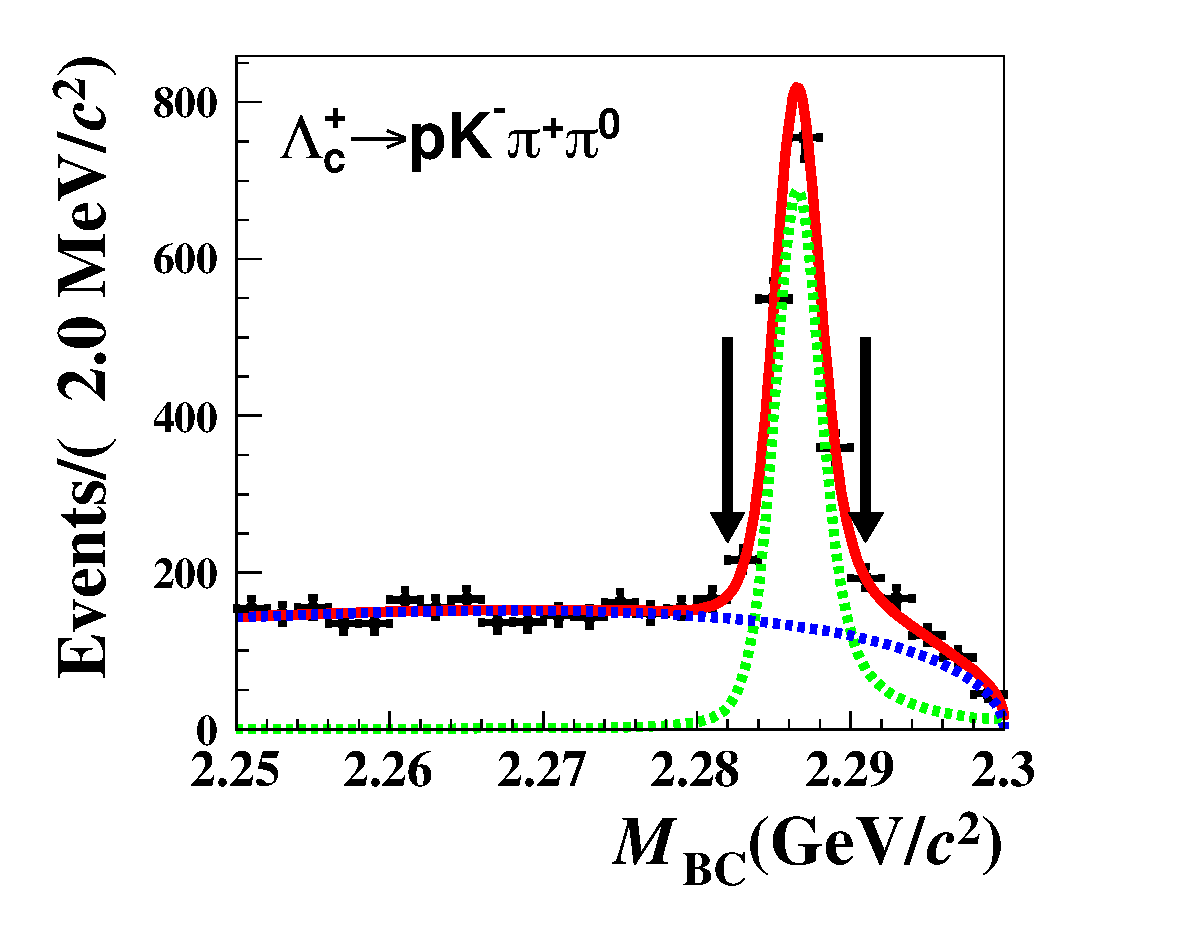
\includegraphics[width=0.3\textwidth]{chap2_ST_data_mode4}
}
\hspace{1pt}
\subfigure[]
{
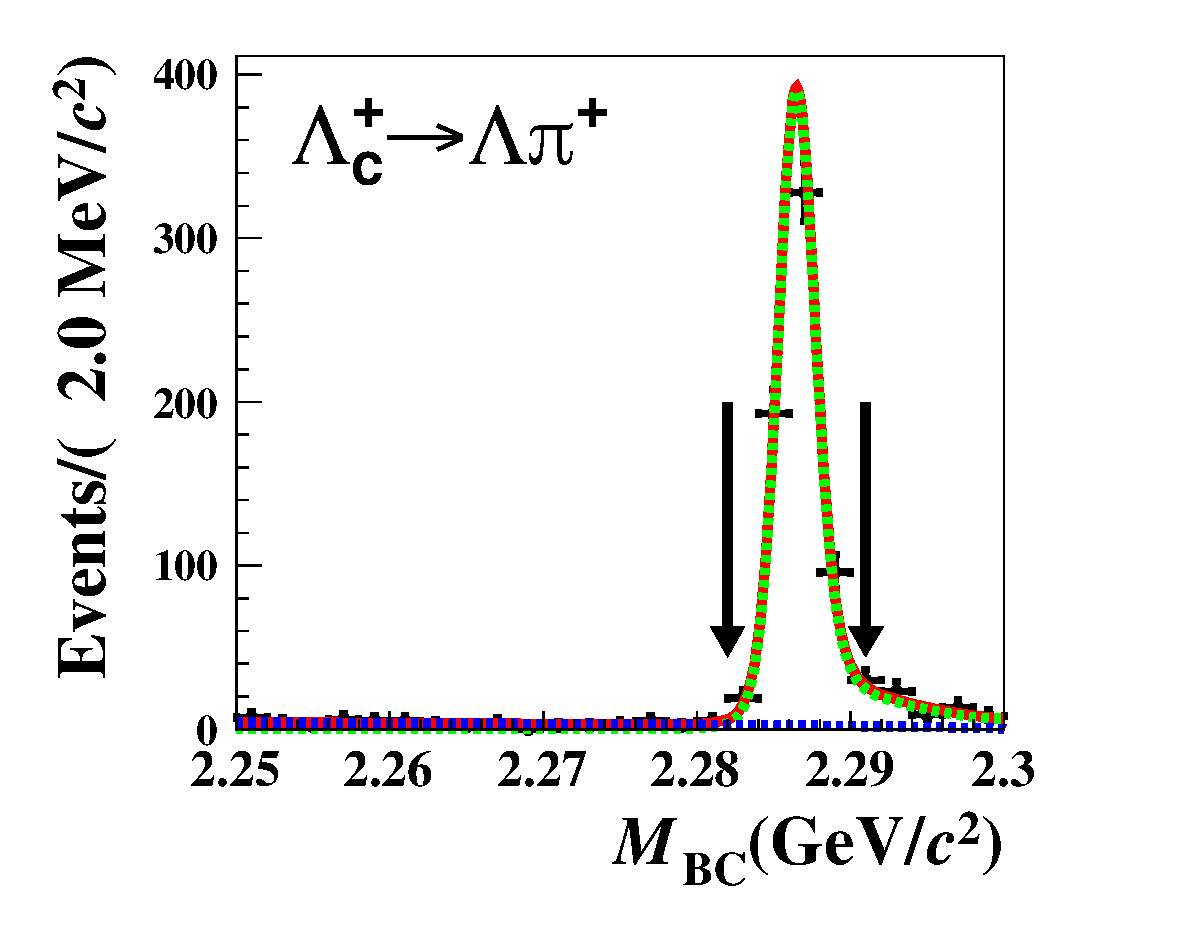
\includegraphics[width=0.3\textwidth]{chap2_ST_data_mode30}
}
\hspace{1pt}
\subfigure[]
{
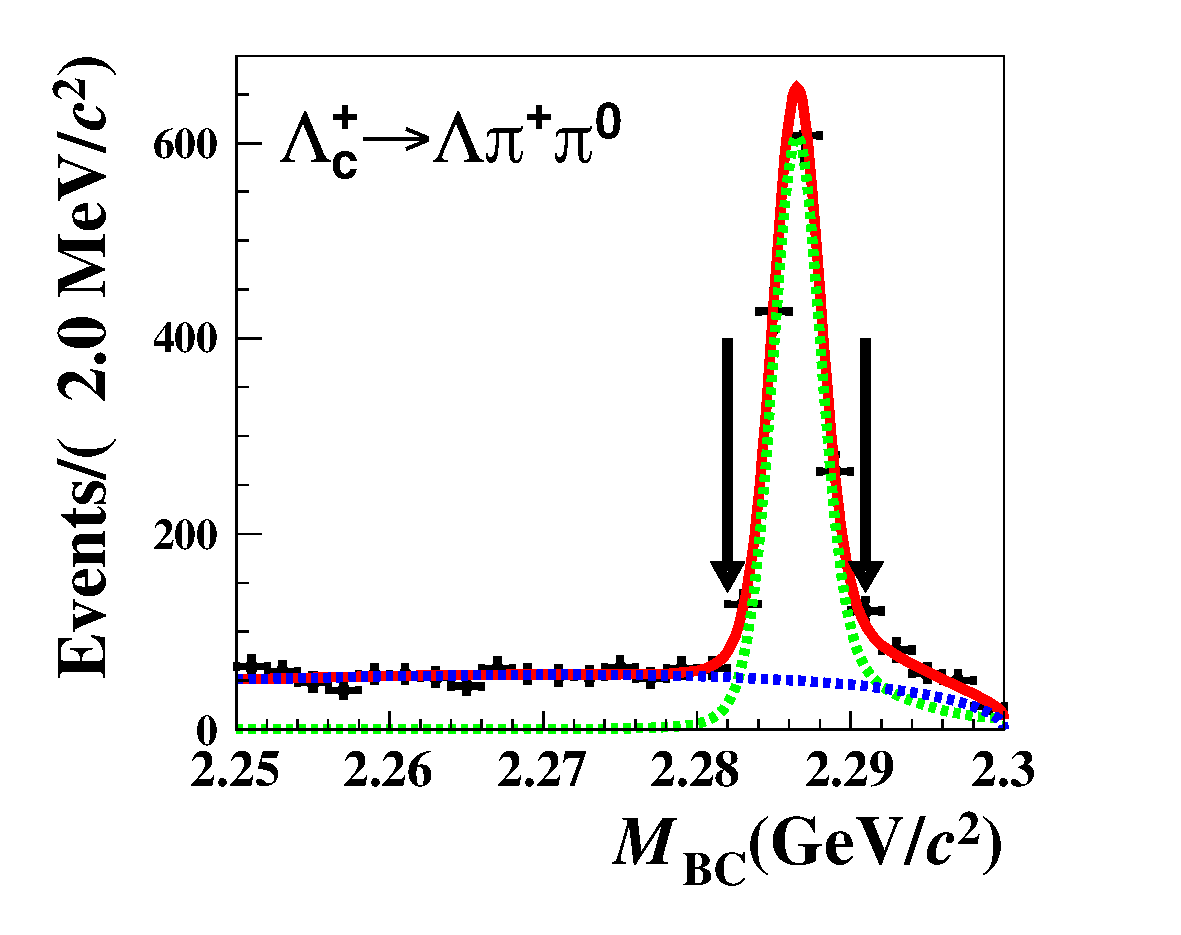
\includegraphics[width=0.3\textwidth]{chap2_ST_data_mode31}
}
\hspace{2pt}
\subfigure[]
{
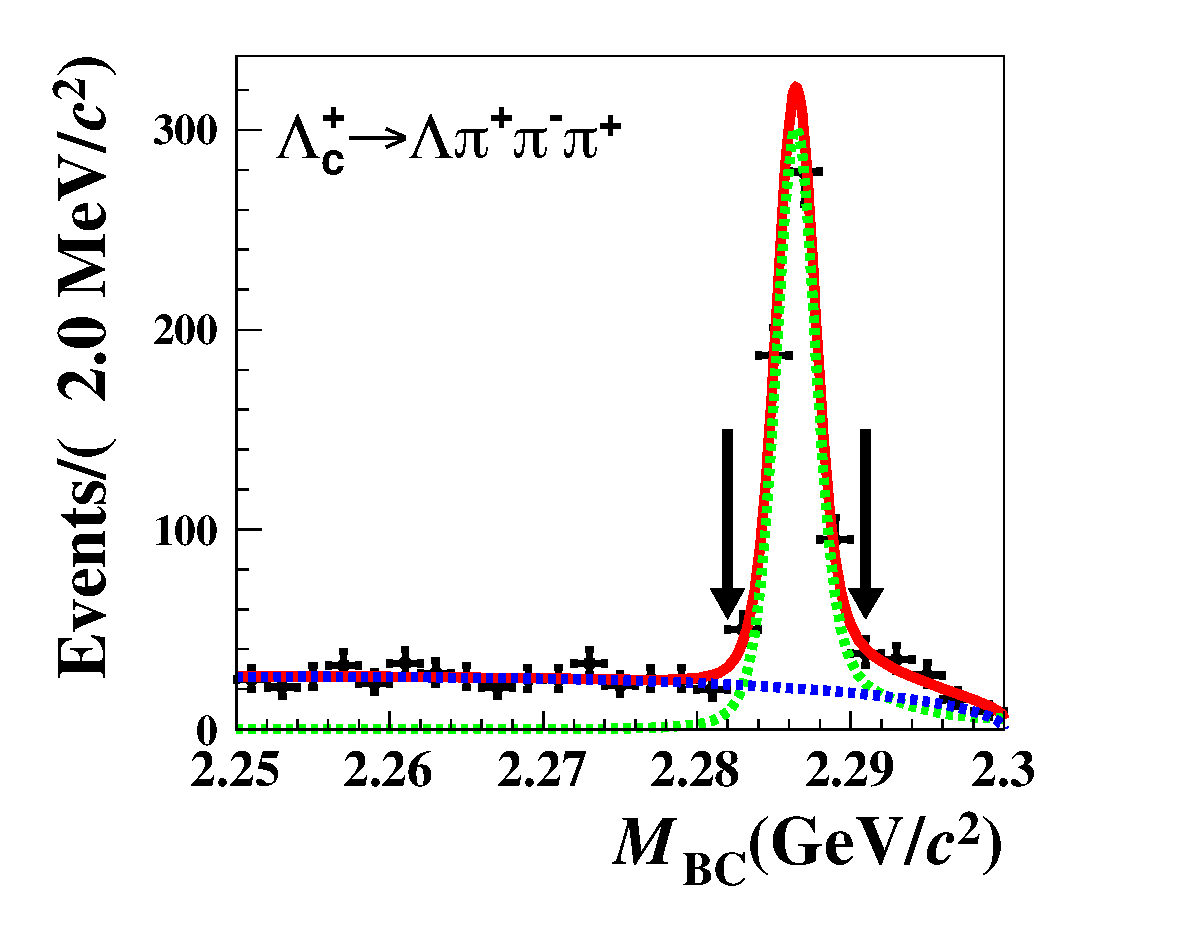
\includegraphics[width=0.3\textwidth]{chap2_ST_data_mode33}
}
\hspace{1pt}
\subfigure[]
{
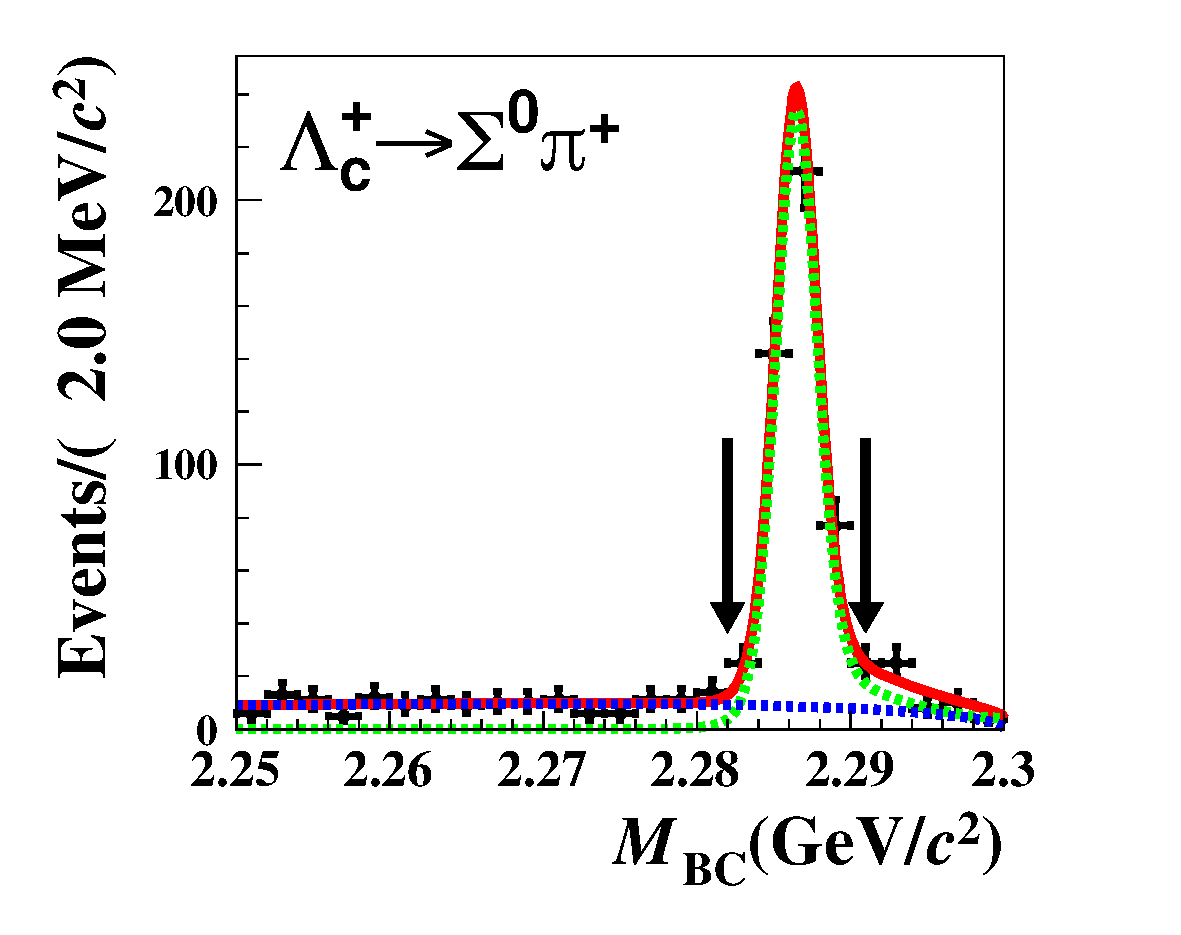
\includegraphics[width=0.3\textwidth]{chap2_ST_data_mode60}
}
\hspace{1pt}
\subfigure[]
{
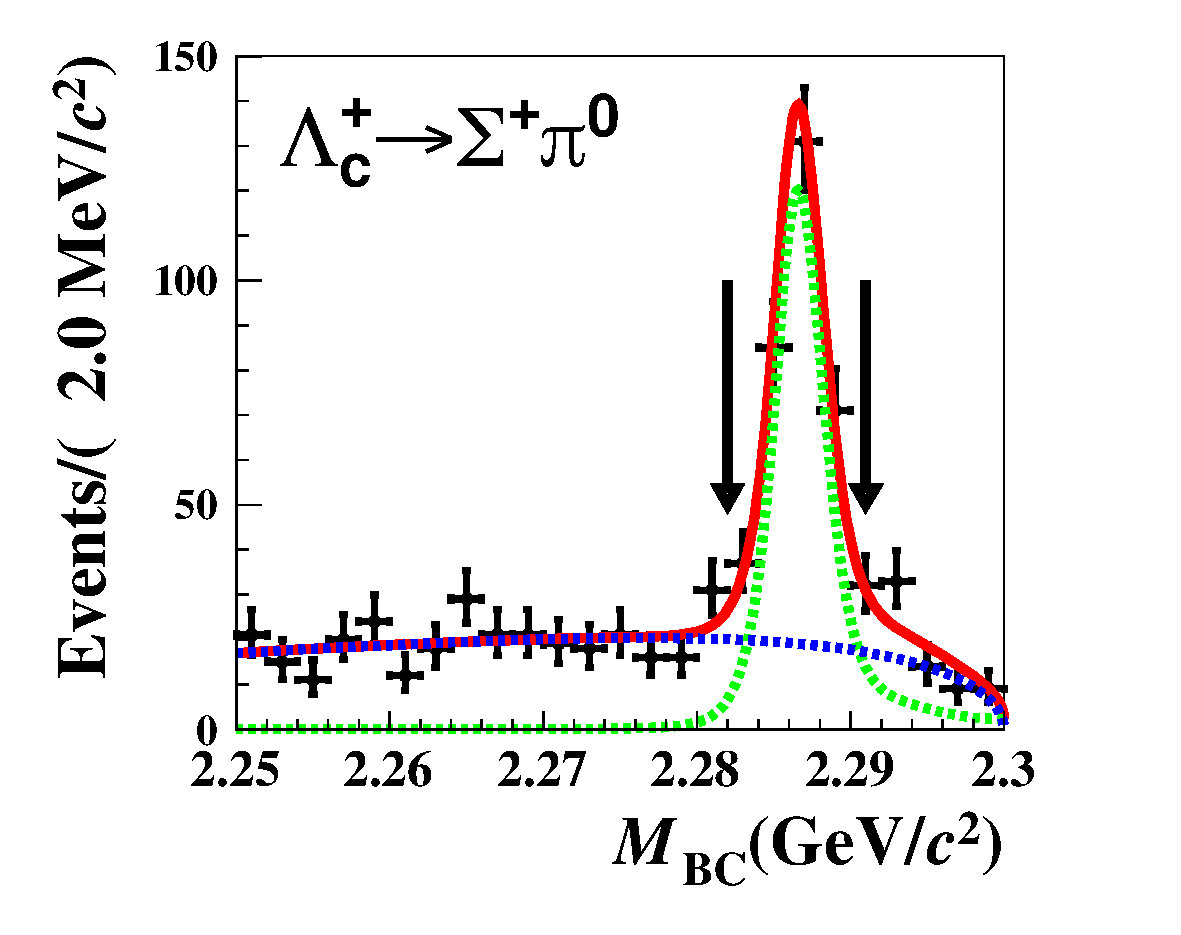
\includegraphics[width=0.3\textwidth]{chap2_ST_data_mode62}
}
\hspace{1pt}
\subfigure[]
{
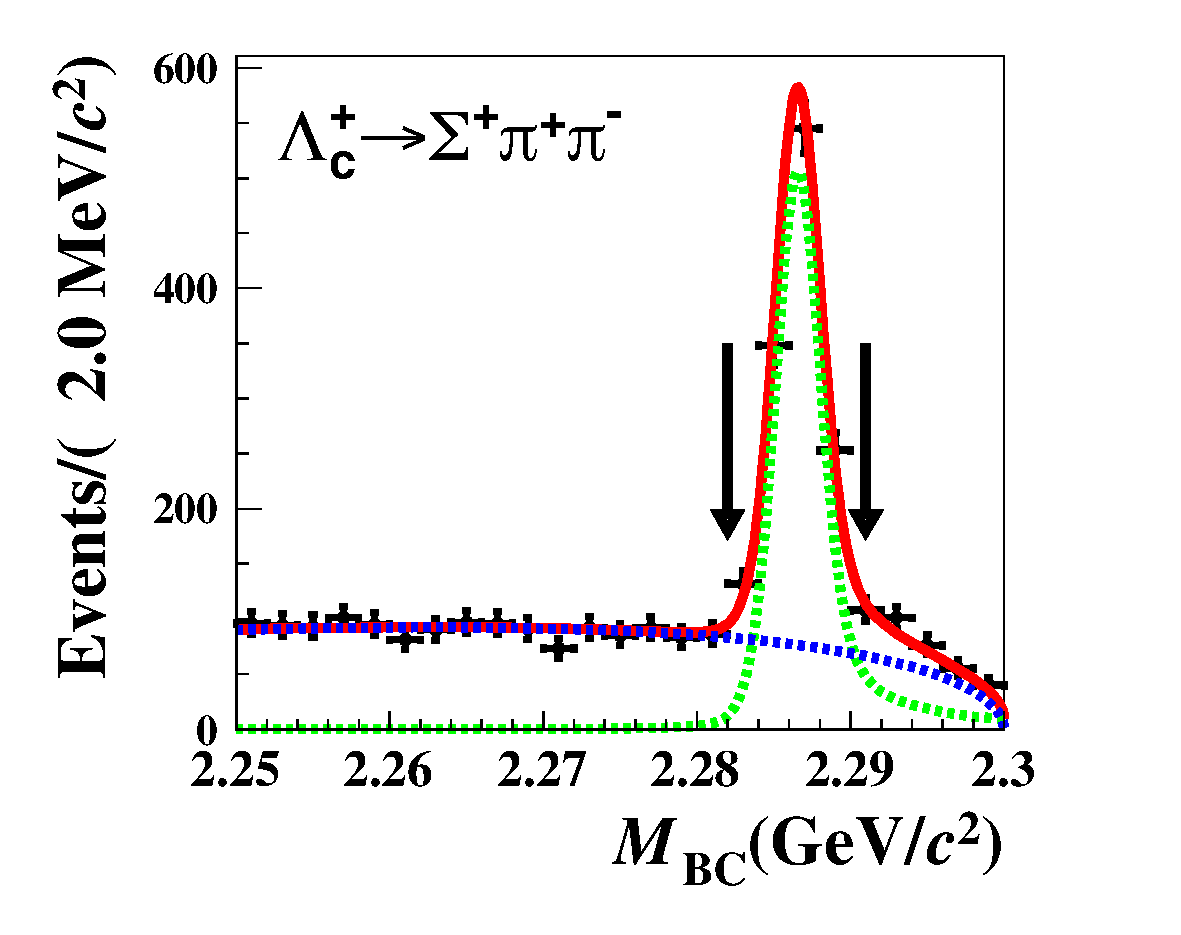
\includegraphics[width=0.3\textwidth]{chap2_ST_data_mode63}
}
\hspace{1pt}
\subfigure[]
{
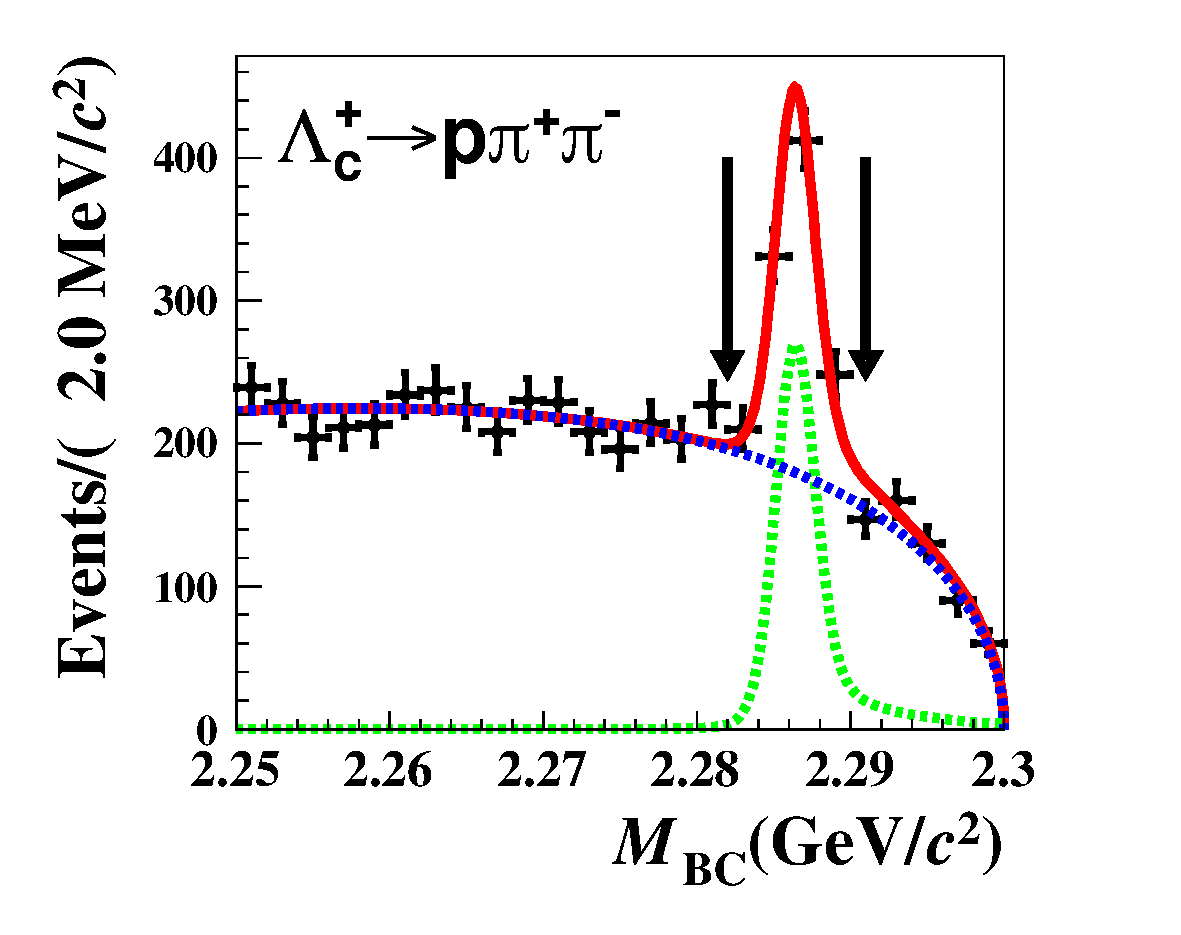
\includegraphics[width=0.3\textwidth]{chap2_ST_data_mode5}
}
\caption{拟合\textbf{数据}中单标记~$M_{\rm BC}$分布得产额的拟合结果,每个道的~$\lambdacp$ 及~$\lambdacm$ 均合在一起拟合。在每个图中,黑色的带误差的点代表数据的分布,红色实的曲线是拟合结果,绿色虚线是信号的形状,蓝色虚线是本底ARGUS函数分布。}
\label{fig:ST_datafit}
\end{figure*}


%%%%%%%%%%%%%%%%%%%%%%%%%%%%
\begin{figure*}[]
\centering
\subfigure[]
{
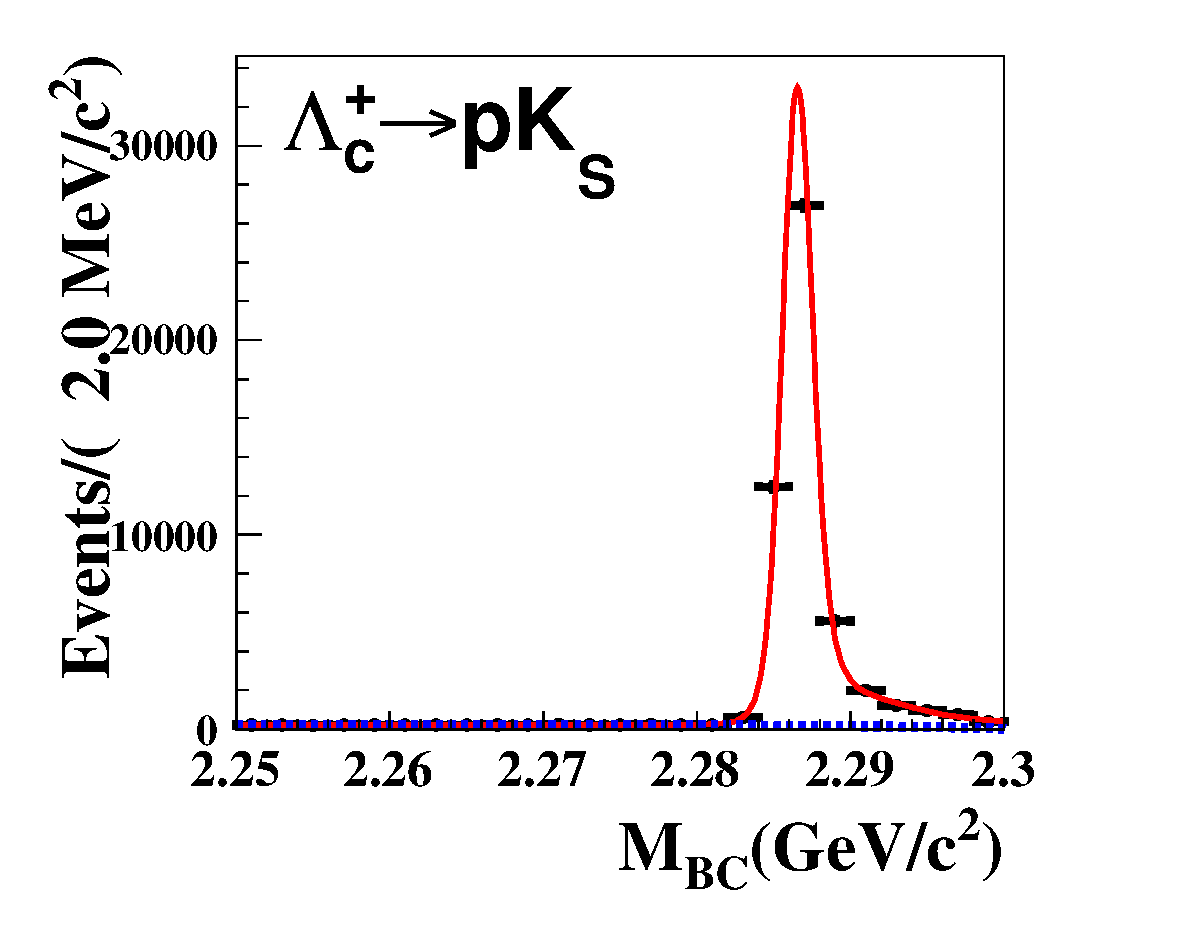
\includegraphics[width=0.3\textwidth]{chap2_ST_cockmc_mode0}
}
\hspace{1pt}
\subfigure[]
{
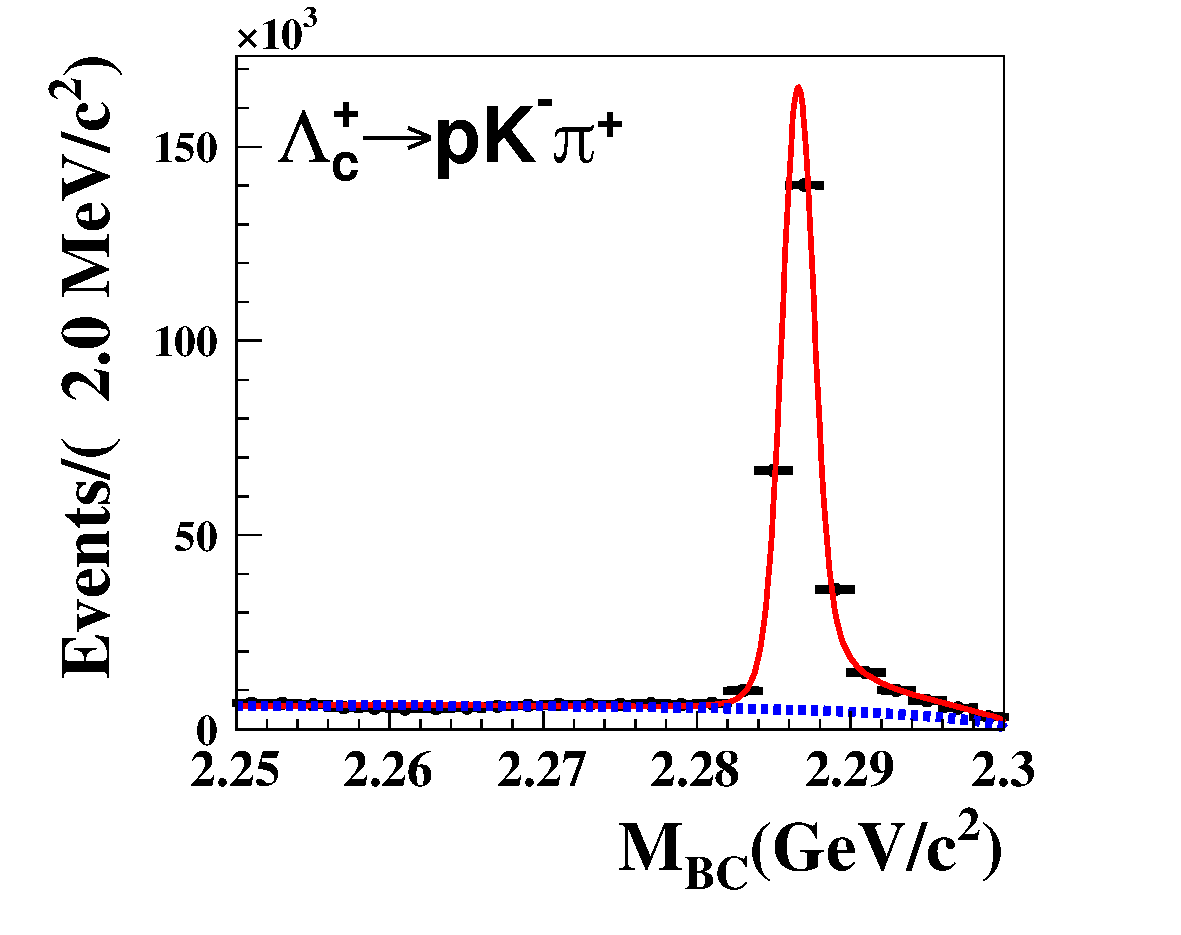
\includegraphics[width=0.3\textwidth]{chap2_ST_cockmc_mode1}
}
\hspace{1pt}
\subfigure[]
{
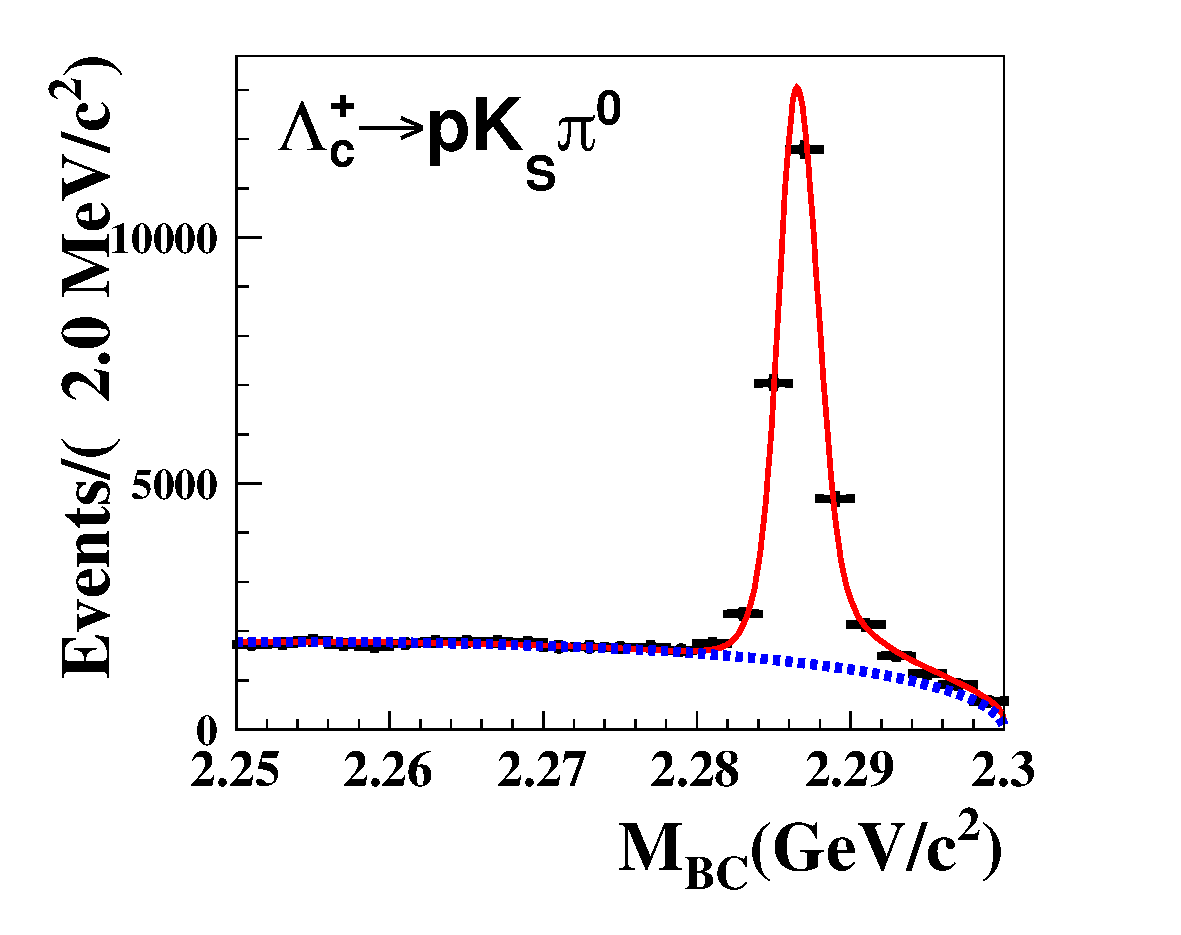
\includegraphics[width=0.3\textwidth]{chap2_ST_cockmc_mode2}
}
\hspace{1pt}
\subfigure[]
{
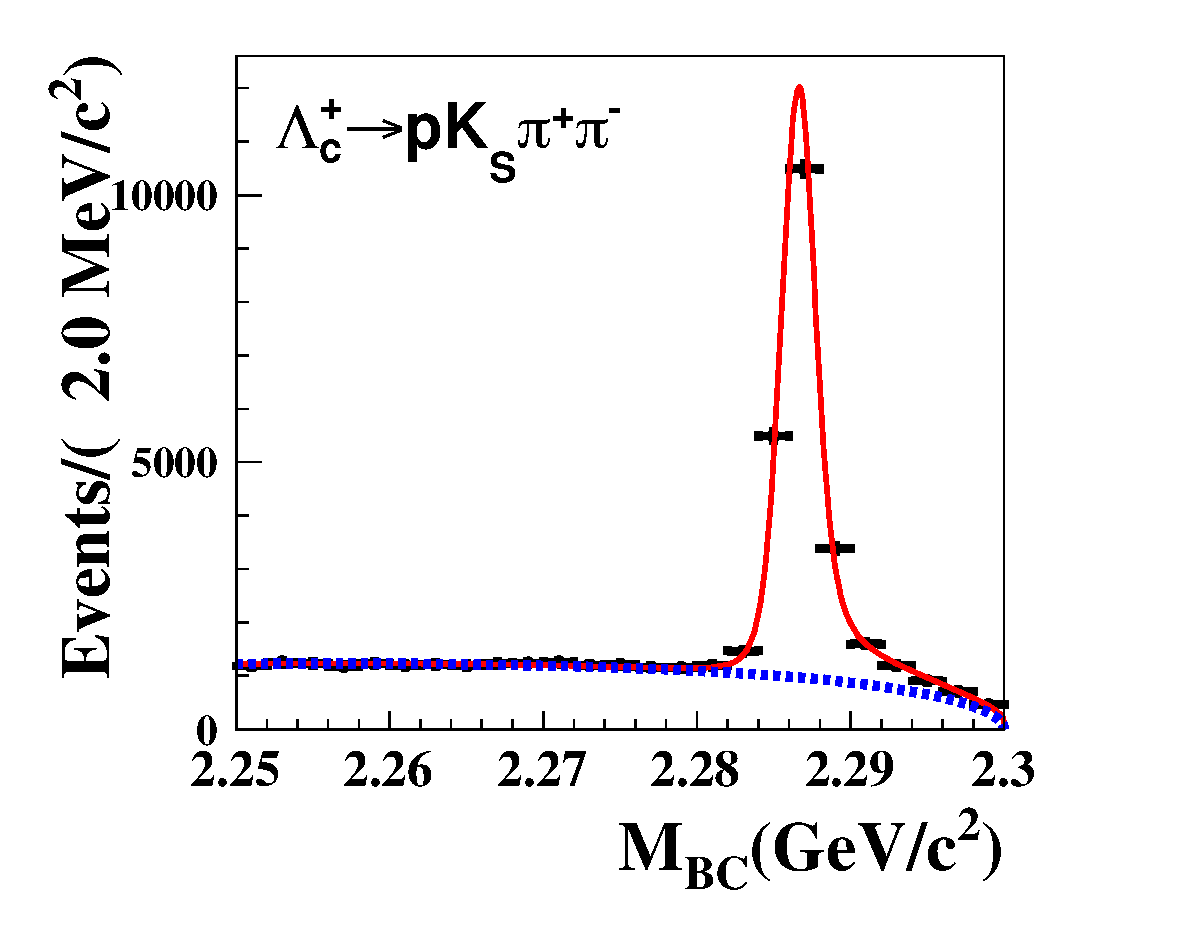
\includegraphics[width=0.3\textwidth]{chap2_ST_cockmc_mode3}
}
\hspace{1pt}
\subfigure[]
{
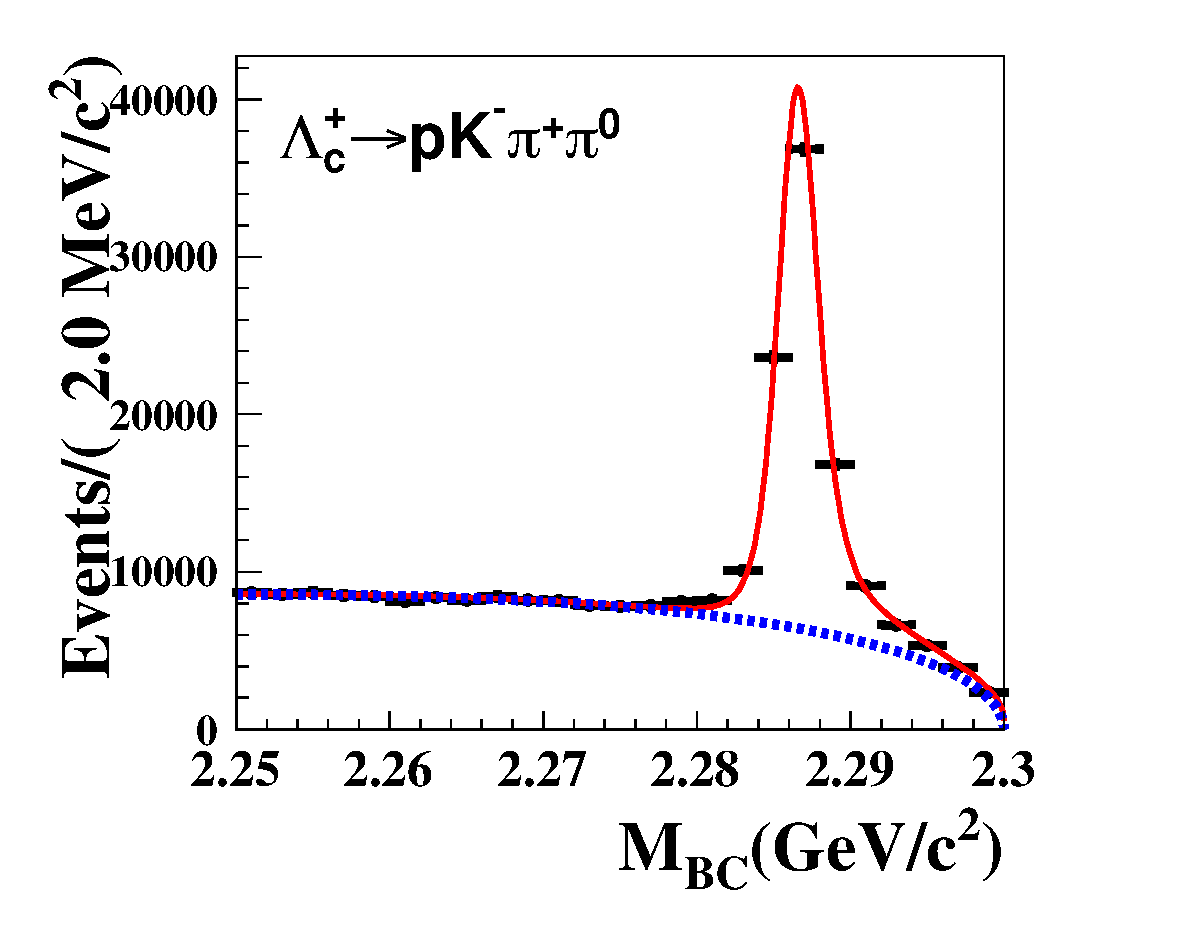
\includegraphics[width=0.3\textwidth]{chap2_ST_cockmc_mode4}
}
\hspace{1pt}
\subfigure[]
{
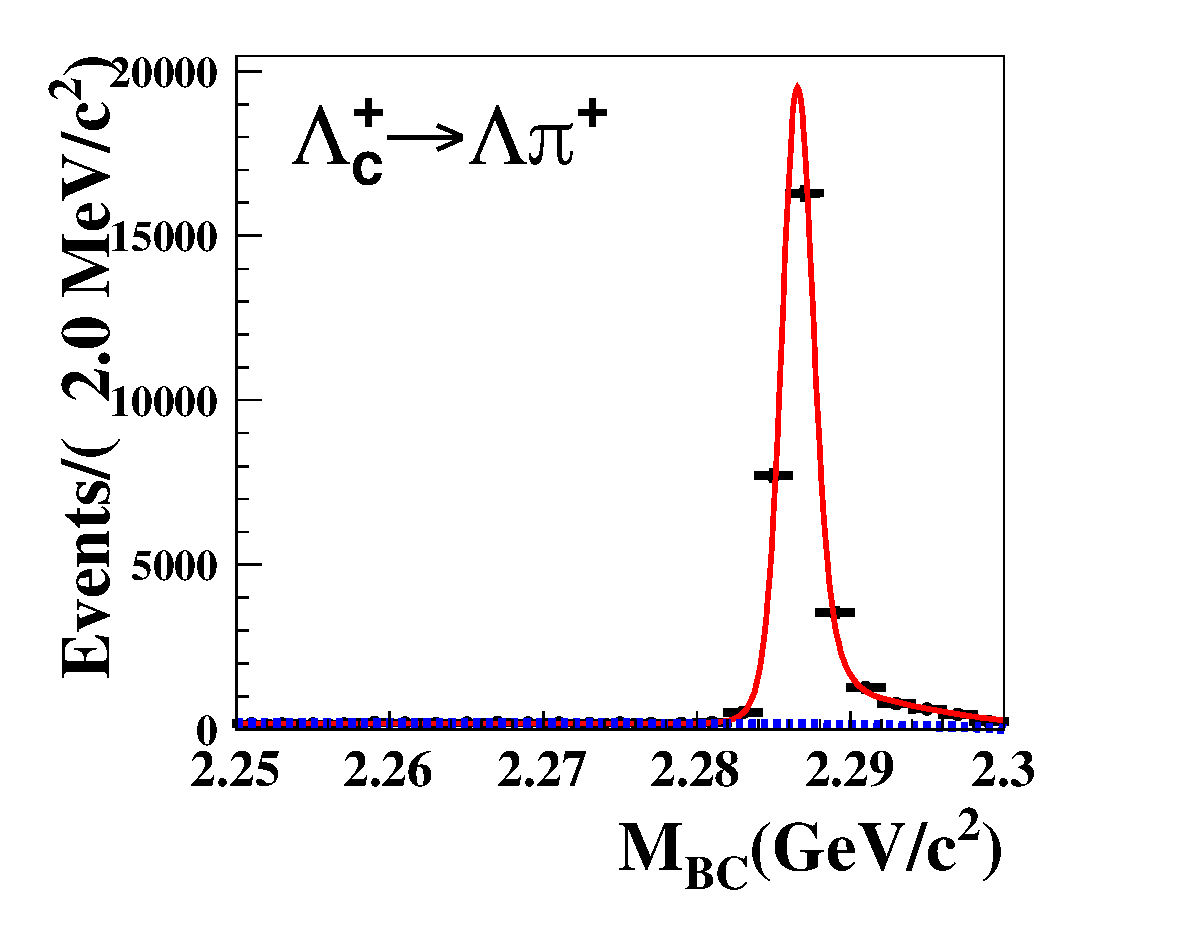
\includegraphics[width=0.3\textwidth]{chap2_ST_cockmc_mode30}
}
\hspace{1pt}
\subfigure[]
{
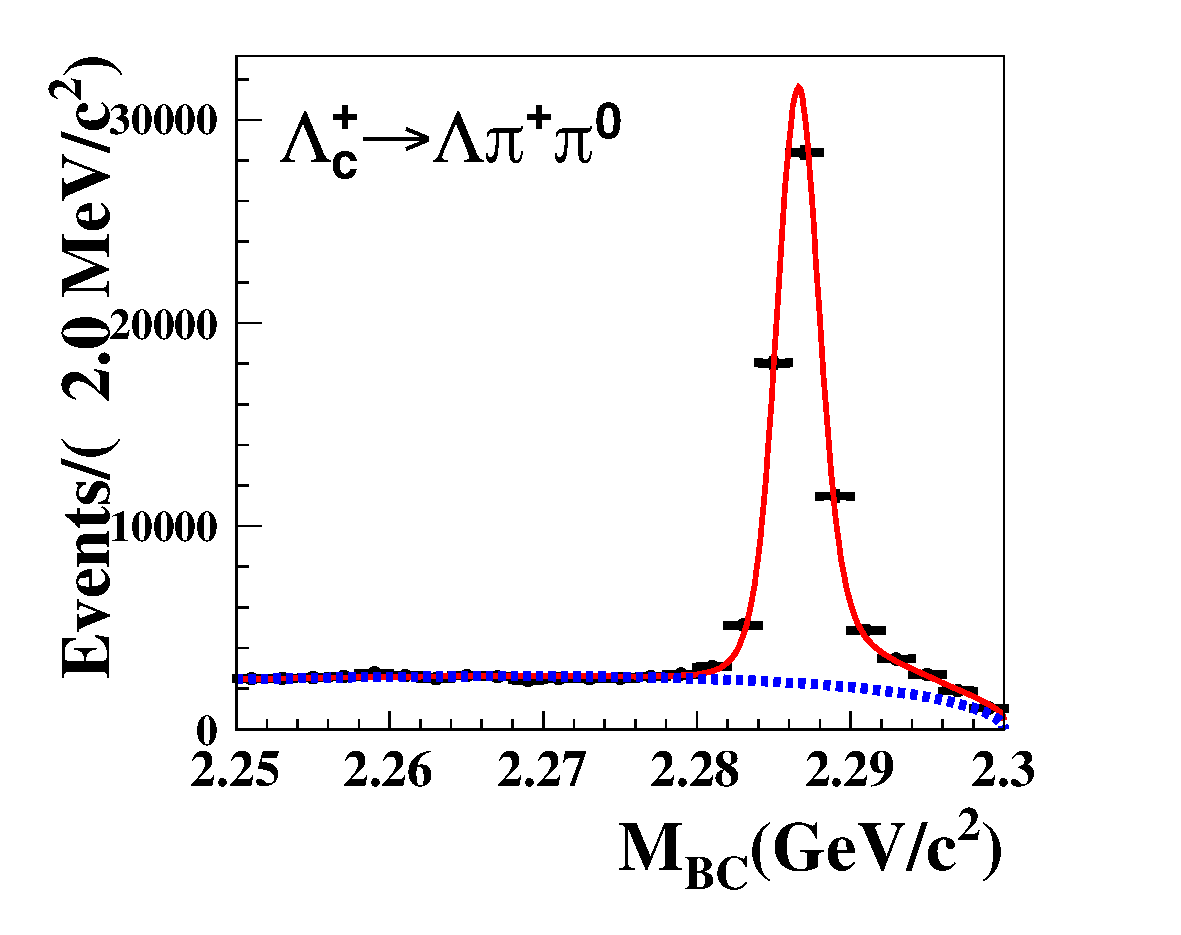
\includegraphics[width=0.3\textwidth]{chap2_ST_cockmc_mode31}
}
\hspace{1pt}
\subfigure[]
{
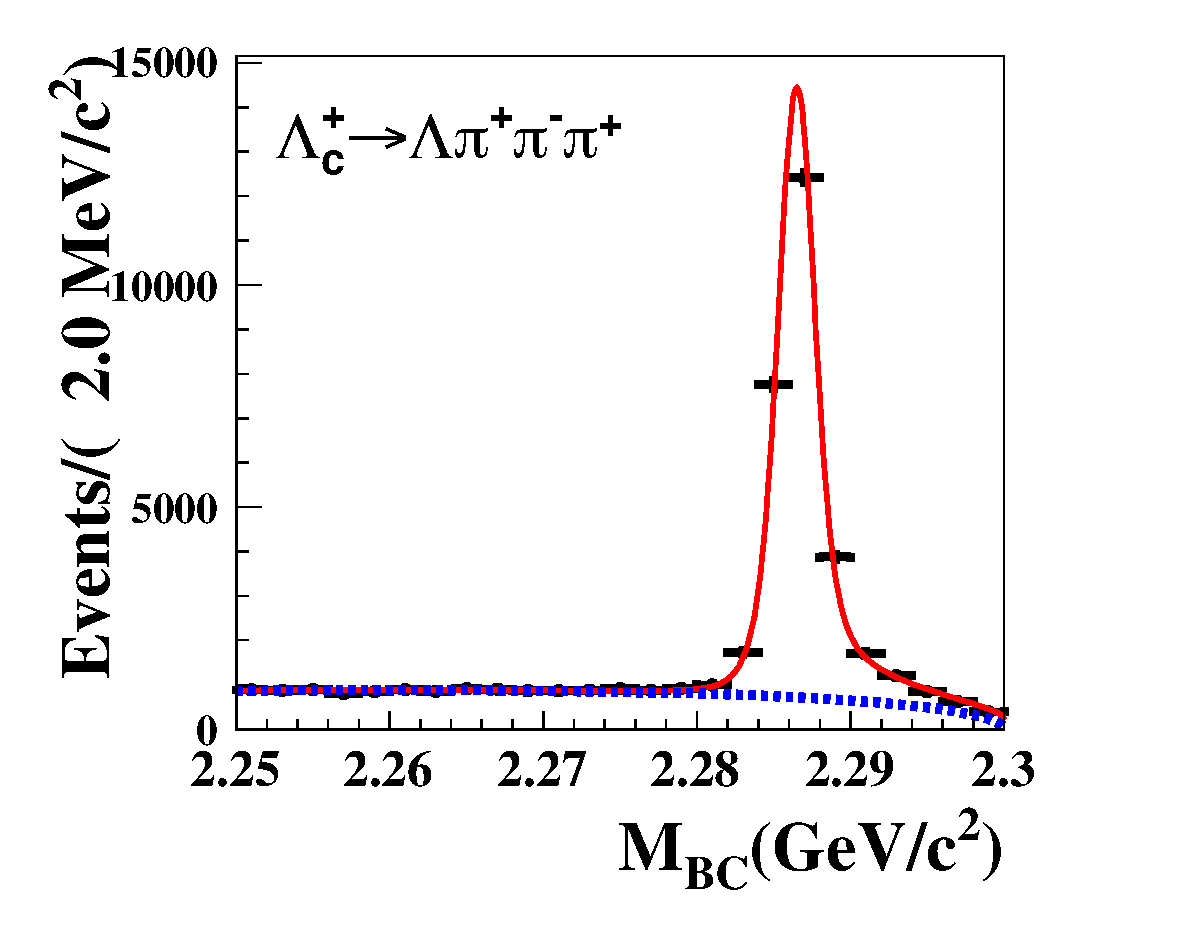
\includegraphics[width=0.3\textwidth]{chap2_ST_cockmc_mode33}
}
\hspace{1pt}
\subfigure[]
{
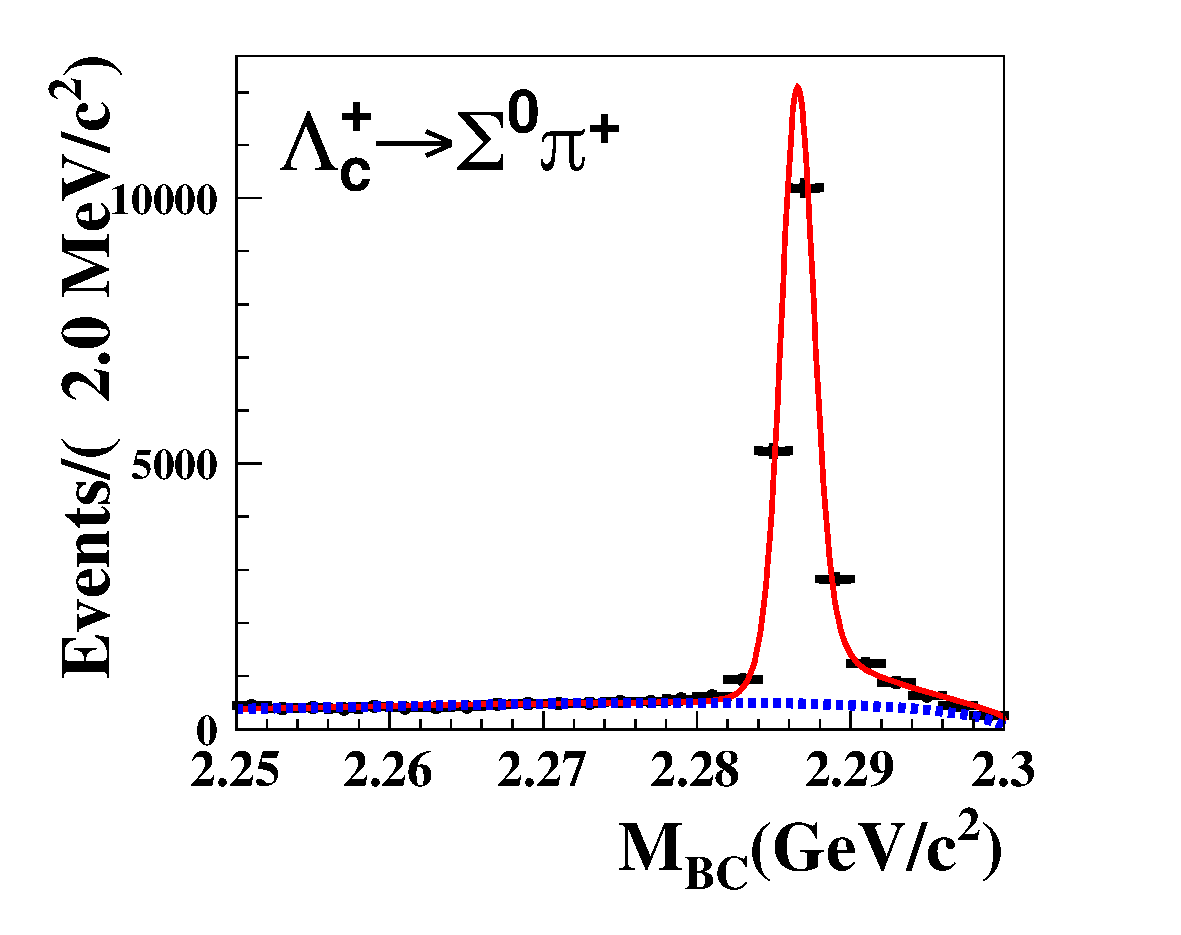
\includegraphics[width=0.3\textwidth]{chap2_ST_cockmc_mode60}
}
\hspace{1pt}
\subfigure[]
{
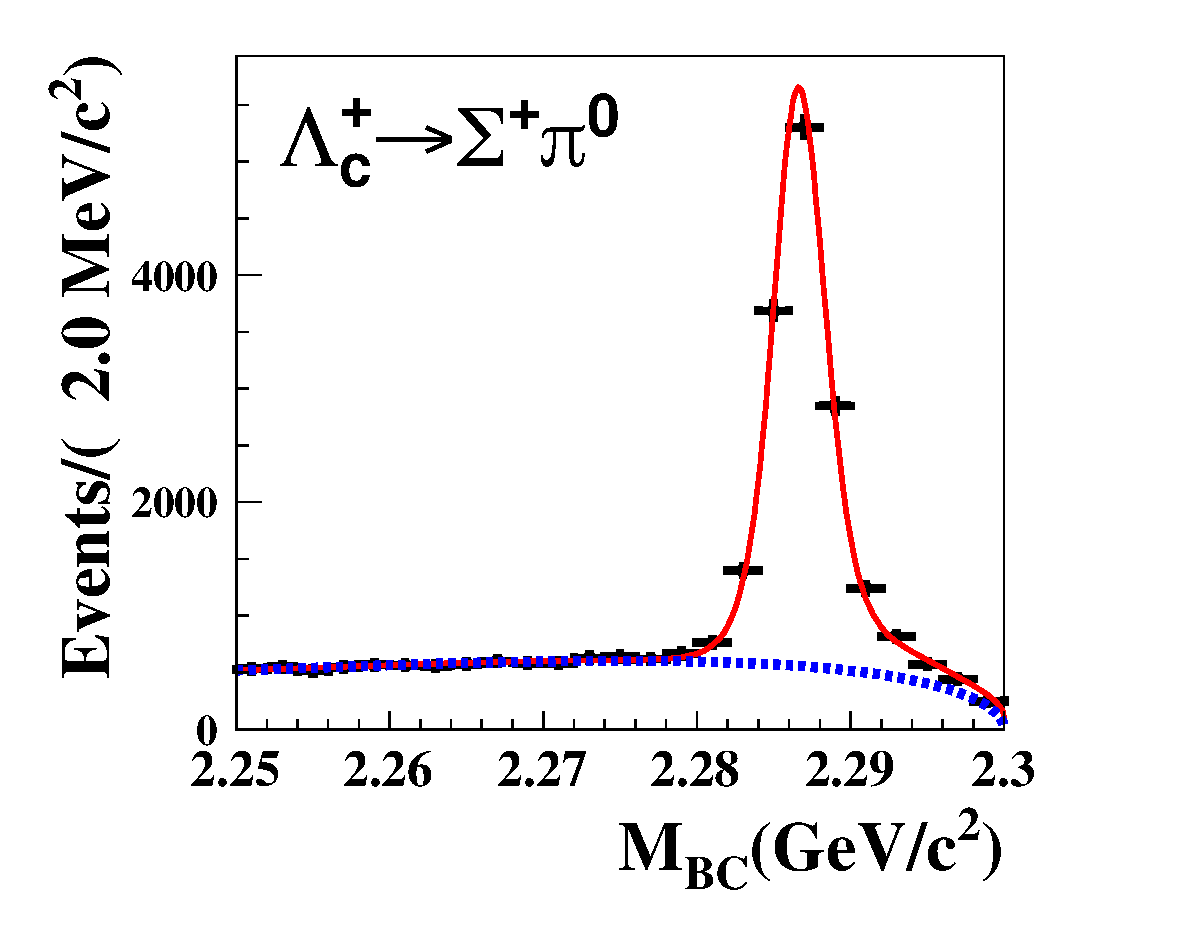
\includegraphics[width=0.3\textwidth]{chap2_ST_cockmc_mode62}
}
\hspace{1pt}
\subfigure[]
{
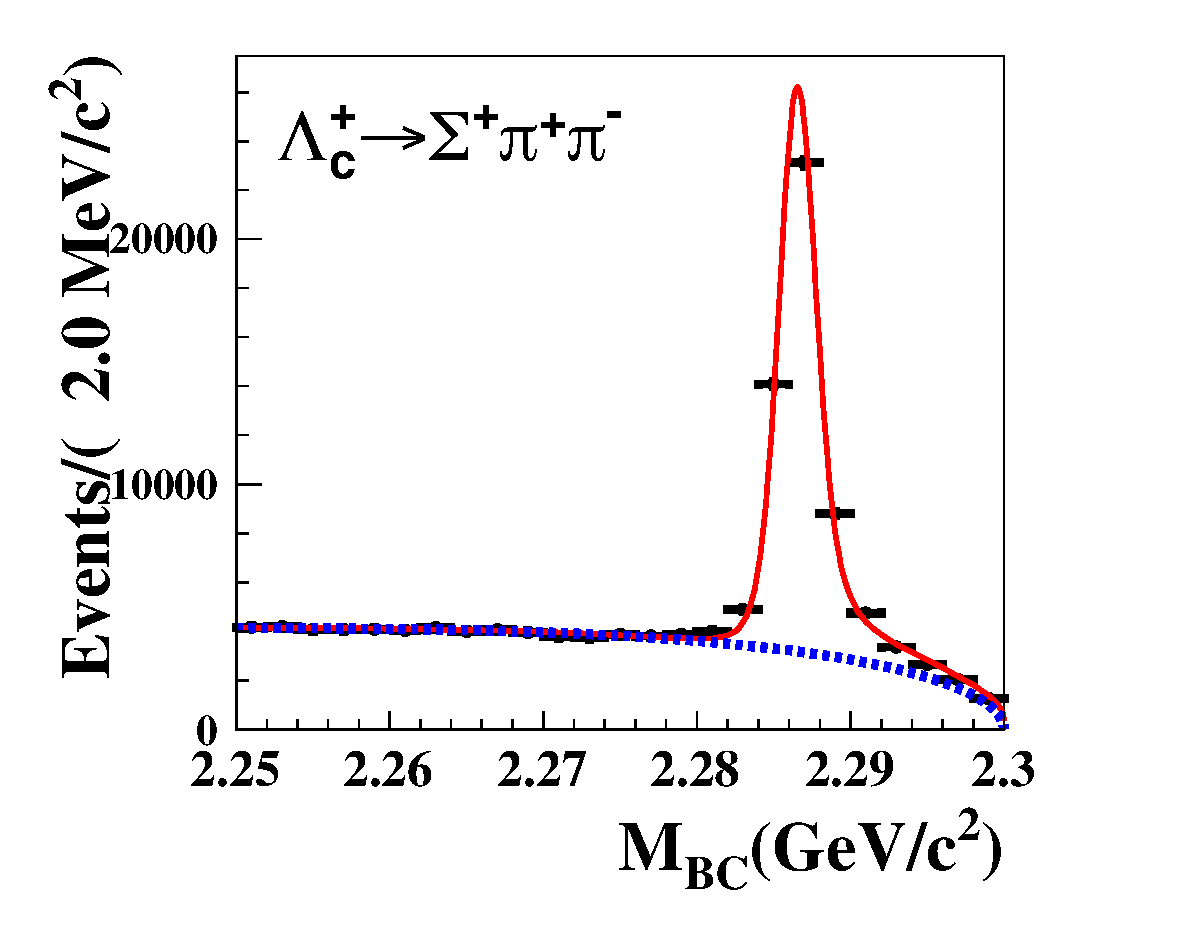
\includegraphics[width=0.3\textwidth]{chap2_ST_cockmc_mode63}
}
\hspace{1pt}
\subfigure[]
{
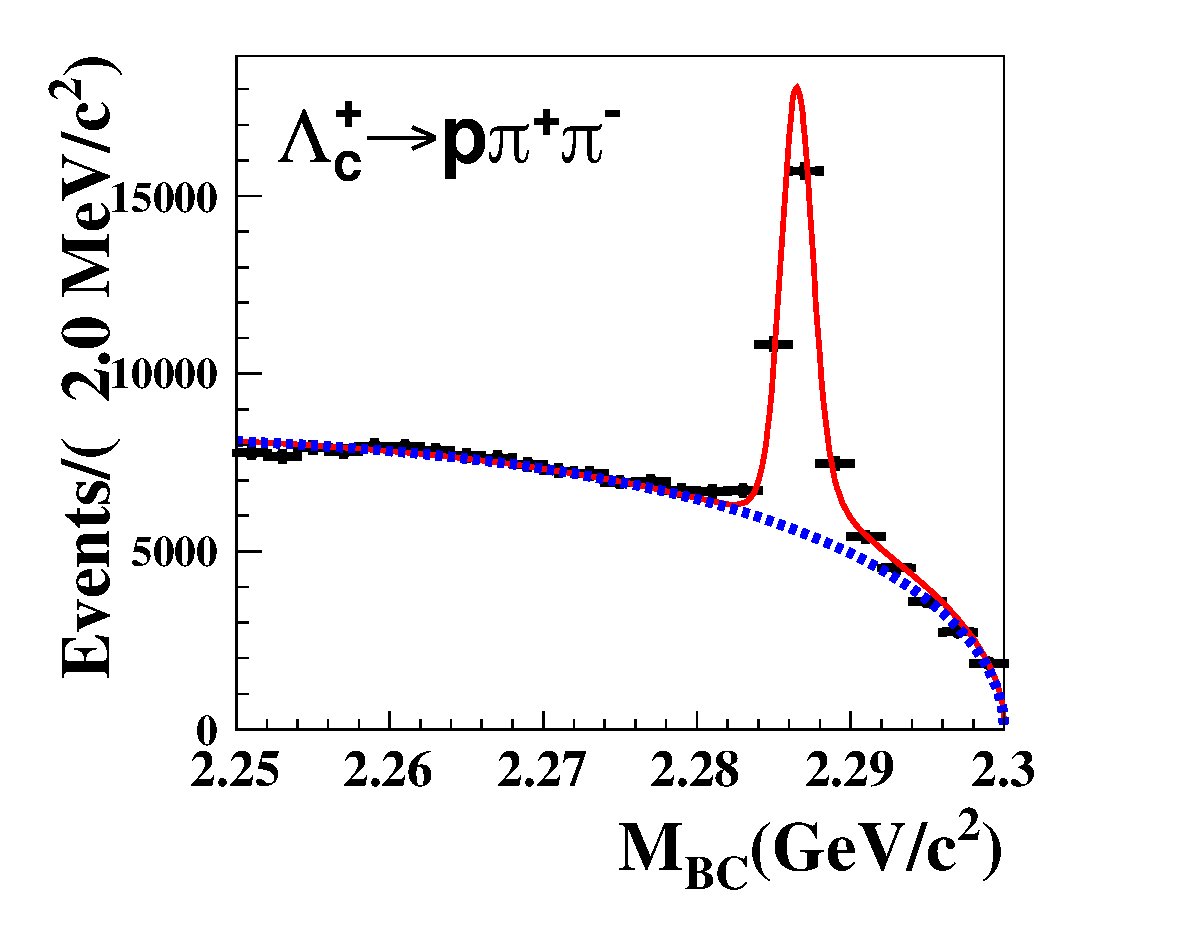
\includegraphics[width=0.3\textwidth]{chap2_ST_cockmc_mode5}
}
\caption{拟合\textbf{Cocktail MC}中单标记~$M_{\rm BC}$分布得重建效率的拟合结果,每个道的~$\lambdacp$ 及~$\lambdacm$ 均合在一起拟合。在每个图中,黑色的带误差的点代表数据样本的分布,红色实的曲线是拟合结果,蓝色虚线是本底ARGUS函数分布。}

\label{fig:ST_cockmcfit}
\end{figure*}


